\documentclass{article}

\usepackage{graphicx}
\usepackage{subcaption}
\usepackage{amsmath, amssymb}
\usepackage{bm}
\usepackage{appendix}
\usepackage{float}
\usepackage{tabularx}
\usepackage[section]{placeins}

\begin{document}

\title{\vspace{1cm}Project 3 \\ FYS3150}

\author{\vspace{1cm}Ann-Silje Kirkvik \\ github.com/annsilje/fys3150}
\date{\vspace{5cm}\today}

\maketitle

\newpage

\begin{abstract}
This project models the orbits of the planets and the Sun in the solar system by numerically solving coupled ordinary differential equations describing the motion of the celestial bodies based on the gravitational force. For the Earth-Sun system the numerical algorithms Forward Euler and Velocity Verlet have been tested. The Velocity Verlet algorithm turned out to perform significantly better than the Forward Euler algorithm and is the preferred choice for simulating the orbits. Both algorithms scale linearly with the number of integration points, but the Forward algorithm requires fewer floating point operations and is therefore slightly faster. The three-body problem of the Earth-Jupiter-Sun system has been simulated with different masses for the planet Jupiter, and the 9-body problem of the solar system has been solved. The Sun is the by far most important contributor to the planets' orbits, but the planets also have an effect on the motion of the Sun, which again affects the motion of the planets. Finally, a modified Newtonian gravitational force with a correction to account for the effects of general relativity is tested to investigate the impact on Mercury's orbit. The discrepancy between the expected precession of Mercury's orbit from the classical newtonian gravitational force of the other celestial bodies in the solar system and the observed value can be reproduced with the modified Newtonian gravitational force.
\end{abstract}

\vspace{1cm}


\section{Introduction}
This project models the orbits of the planets and the Sun in the solar system by numerically solving coupled ordinary differential equations describing the motion of the celestial bodies based on the gravitational force. To solve these equations numerically the Forward Euler and Velocity Verlet methods are tested, with emphasis on the latter. Several scenarios are tested, ranging from the two-body problem of the Earth-Sun system to the 9-body problem of all planets and the star of the solar system. In addition, a modified gravitational force model is tested for the two-body problem of the Mercury-Sun system to look at the effects of general relativity on the planet's orbit. Section \ref{sec:description} describes the theoretical background of the project and implementation. Section \ref{sec:results} shows the results of the numerical experiments and section \ref{sec:conclusions} has some final remarks.


\section{Description}
\label{sec:description}
Newton's law of gravitation describes the gravitational force exerted on a body by another body and is given by

\begin{equation}
\bm{F}_{12} = \frac{Gm_1m_2}{r^3}\bm{r}
\end{equation}
where $G$ is the gravitational constant, $m_1$ and $m_2$ are the masses of the two bodies involved, $\bm{r} = \bm{x_2} - \bm{x_1}$, where $\bm{x}_k$ is the position vector of body $k$ and $r$ is the relative distance between the bodies. By applying Newton's second and third laws of motion, $\Sigma\bm{F} = m\bm{\ddot x}$ and $\bm{F}_{12}=-\bm{F}_{21}$, the following second order differential equations are obtained

\begin{equation}
\frac{d^2\bm{x}_1}{dt^2} = \frac{\bm{F_}{12}}{m_1} \quad \text{ and } \quad \frac{d^2\bm{x}_2}{dt^2} = \frac{\bm{F}_{21}}{m_2}
\end{equation}
where each equation can be rewritten into a set of first order differential equations:

\begin{equation}
\frac{d\bm{x}}{dt} = \bm{v} \quad \text{ and } \quad \frac{d\bm{v}}{dt} = \frac{\bm{F}}{m}
\end{equation}

For a two-body problem in three dimensions this leads to 12 coupled first order differential equations. For the three-body problem in three dimensions the number of equations increases to 18. In general, there are 6 coupled first order differential equations for each body. For the 9-body problem of the solar system this becomes 54 equations. Each equation also has an initial condition for the time $t_0=0$, yielding the initial position and velocity of each body. Since the Sun is large compared to the other celestial bodies, it can be reasonable in some cases to ignore the forces the planets exert on the Sun and keep the Sun's position fixed. This will reduce the number of equations by 6 for each case.

Choosing a step size, $h$, and discretizing the problem with $t_{i+1} = t_i + ih$, for $i=0,1,...,n$, these differential equations can be solved numerically using numerous different methods. Here, only two of these methods will be tested, namely the Forward Euler and Velocity Verlet algorithms, which is also described in \cite{lectures}.

\subsection{Forward Euler}
\label{sec:euler}
Making a Taylor expansion of the position and velocity vectors $\bm{x}$ and $\bm{v}$ gives

\begin{equation}
\bm{x}(t_{i+1}) = \bm{x}_{i+1} = \bm{x}_i + h\frac{d\bm{x}_i}{dt} + \mathcal{O}(h^2)
\end{equation}
\begin{equation} 
\bm{v}(t_{i+1}) = \bm{v}_{i+1} = \bm{v}_i + h\frac{d\bm{v}_i}{dt} + \mathcal{O}(h^2)
\end{equation} 
This gives the Forward Euler algorithm:
\begin{enumerate}
\item $\bm{a}_i = \Sigma\bm{F}_i/m$
\item $\bm{v}_{i+1} = \bm{v}_i + h\bm{a}_i$
\item $\bm{x}_{i+1} = \bm{x}_i + h\bm{v}_i$
\end{enumerate}
where the acceleration $\bm{a}_i$ is determined by Newton's second law. The local error of the Forward Euler algorithm goes as $\mathcal{O}(h^2)$ and the updated positions and velocities are linear extrapolations from the previous step. The advantage of this algorithm though, is its simplicity. Updating the positions require 2 floating point operations for each dimension, and the same is required for updating the velocities.

\subsection{Velocity Verlet}
\label{sec:verlet}
Again, starting with a Taylor expansion of the position and velocity vectors $\bm{x}$ and $\bm{v}$, but also the acceleration vector $\bm{a}$:

\begin{equation}
\bm{x}(t_{i+1}) = \bm{x}_{i+1} = \bm{x}_i + h\frac{d\bm{x}_i}{dt} + \frac{h^2}{2}\frac{d^2\bm{x}_i}{dt^2} + \mathcal{O}(h^3)
\end{equation}
\begin{equation} 
\bm{v}(t_{i+1}) = \bm{v}_{i+1} = \bm{v}_i + h\frac{d\bm{v}_i}{dt} + \frac{h^2}{2}\frac{d^2\bm{v}_i}{dt^2} + \mathcal{O}(h^3)
\label{eq:vel}
\end{equation} 
\begin{equation} 
\bm{a}(t_{i+1}) = \bm{a}_{i+1} = \bm{a}_i + h\frac{d\bm{a}_i}{dt} + \mathcal{O}(h^2)
\label{eq:acc}
\end{equation}
Solving equation \ref{eq:acc} for $h\frac{d\bm{a}_i}{dt} = h\frac{d^2\bm{v}_i}{dt^2}$ and inserting into equation \ref{eq:vel} gives 

\begin{flalign}
\nonumber\bm{v}_{i+1} &= \bm{v}_i +  h\frac{d\bm{v}_i}{dt} + \frac{h}{2}(\bm{a}_{i+1} - \bm{a}_i) + \mathcal{O}(h^3) \\
&= \bm{v}_i + \frac{h}{2}(\bm{a}_i + \bm{a}_{i+1}) + \mathcal{O}(h^3)
\end{flalign} 
The Velocity Verlet algorithm then becomes:
\begin{enumerate}
\item $\bm{a}_i = \Sigma\bm{F}_i/m$
\item $\bm{x}_{i+1} = \bm{x}_i + h\bm{v}_i + h^2\bm{a}_i/2$
\item $\bm{a}_{i+1} = \Sigma\bm{F}_{i+1}/m$
\item $\bm{v}_{i+1} = \bm{v}_i + h(\bm{a}_i + \bm{a}_{i+1})/2$
\end{enumerate}
where the accelerations $\bm{a}_i$ and $\bm{a}_{i+1}$ are determined by Newton's second law, and $\bm{F}$ depends on the position of the bodies. The Velocity Verlet algorithm has a local error that goes as $\mathcal{O}(h^3)$, which is an improvement over the Forward Euler algorithm. In addition, the updated position now also takes into account the acceleration at the previous position and the velocity is updated using the average acceleration over the time step $[t_i, t_{i+1}]$. 

Updating the positions require 5 floating point operations for each dimension, and updating the velocities require 4 floating point operations for each dimension. Since the step size is constant these numbers can be reduced to 4 and 3 respectively by computing the constants $h^2/2$ and $h/2$ only once. Still, this is slightly more operations than in Forward Euler, but both algorithms scale linearly with the number of steps. The Velocity Verlet algorithm is also slightly more complicated because the accelerations and velocities from the previous step need to saved. 

\subsection{Scaling and assumptions}
Distances in space are very large compared to here on Earth and selecting a different unit to measure distances seem appropriate. One such unit is the Astronomical Unit (AU) where 1 AU is the average distance between the Earth and the Sun, which is close to $1.5\times 10^{11}$meter. To measure time year is selected as the unit, with 365.25 days per year and 86400 seconds per day, which is also the time the Earth takes to do one revolution around the Sun. Under the assumption of uniform circular orbits the speed and acceleration of the Earth can be expressed as 

\begin{equation}
v = \frac{2\pi r}{T} 
\label{eq:vel_earth}
\end{equation}

\begin{equation}
a = \frac{v^2}{r} = \frac{F}{M_{Earth}} = \frac{GM_{\odot}}{r^2}
\label{eq:acc_earth}
\end{equation}
Combining equation \ref{eq:vel_earth} and \ref{eq:acc_earth} yields 

\begin{flalign}
\nonumber \frac{GM_{\odot}}{r} &= \frac{(2\pi r)^2}{T^2} \\
GM_{\odot} = \frac{4\pi^2r^3}{T^2} &= 4\pi^2\frac{AU^3}{yr^2}
\end{flalign}

By selecting the unit of mass as 1 solar mass the physical constant $G$ simply becomes $4\pi^2$ (skipping units). Applying the same conversion to the speed of light it becomes roughly $c=63241$AU/yr. The masses of the bodies in the solar system is listed in \ref{tab:mass}. Initial positions and velocities for the these bodies can be obtained from NASA's websites \cite{horizon} or \cite{eph}, but the latter requires a parser library to read the files. One such library is \cite{jplephem}.

\begin{table}[h]
\centering
\caption{The mass of bodies in the solar system}
\label{tab:mass}
\begin{tabularx}{\textwidth}{X X r X r}
\hline
Body    && Mass ($kg$) & & Mass ($M_{\odot}$) \\
\hline\hline
Sun     && $2\times 10^{30}$   && $1$ \\
Earth   && $6\times 10^{24}$   && $1.20\times 10^{-7}$ \\
Jupiter && $1.9\times 10^{27}$ && $2.45\times 10^{-6}$ \\
Mars    && $6.6\times 10^{23}$ && $3.00\times 10^{-6}$ \\
Venus   && $4.9\times 10^{24}$ && $3.30\times 10^{-7}$ \\
Saturn  && $5.5\times 10^{26}$ && $9.50\times 10^{-4}$ \\
Mercury && $3.3\times 10^{23}$ && $1.65\times 10^{-7}$ \\
Uranus  && $8.8\times 10^{25}$ && $4.40\times 10^{-5}$ \\
Neptune && $1.03\times 10^{26}$&& $5.15\times 10^{-5}$ \\
\hline
\end{tabularx}
\end{table}


\subsection{Conserved quantities}
To assess the quality of the different solvers and different time steps some basic physical laws can be used as tests. These laws are described in various basic textbooks on physics, such as \cite{physics}.

As long as the system is closed and does not interact with bodies outside the system the total energy of the system should always be conserved. The only force involved is the gravitational force and the total energy, $E$, of the N-body system then becomes:

\begin{equation}
E = \sum\limits_{i=0}^N\frac{1}{2}m_iv_i^2 - \sum\limits_{i=0}^N\sum_{j>i}^N \frac{Gm_im_j}{r}
\label{eq:energy}
\end{equation}

The total linear momentum $\bm{P}$ is also a conserved quantity, as long as the net force on the system is zero, and is given by:
\begin{equation}
\bm{P} = \sum\limits_{i=0}^Nm_i\bm{v}_i
\end{equation}

Similarly, the total angular momentum $\bm{L}$ is conserved, as long as the net torque on the system is zero, and is given by:
\begin{equation}
\bm{L} = \sum\limits_{i=0}^N m_i(\bm{r}\times\bm{v})
\end{equation}

under the assumption of circular motion and the celestial bodies being modeled as point masses.

\subsection{Escape Velocity}
A system where the total energy is less than zero is considered a bound system and the bodies will orbit each other. When the energy reaches zero, the system is no longer bound and the bodies will escape each others' gravity fields. With the Earth-Sun system, assuming the Sun is fixed at the origin and $r=1$AU, solving equation \ref{eq:energy} for $E=0$ will yield the escape velocity.

\begin{flalign}
\nonumber E &= 0 \\
\nonumber \frac{1}{2}M_{Earth}v_{Earth}^2 &= \frac{GM_{\odot}M_{Earth}}{r} \\
\nonumber v_{Earth}^2 &= \frac{2GM_{\odot}}{r} \\
\nonumber v_{Earth} &= \sqrt{\frac{2GM_{\odot}}{r}} \\
v_{Earth} &= \sqrt{8\pi^2}AU/yr 
\label{eq:esc}
\end{flalign}

Note that Earth's escape velocity does not depends on the mass of the Earth, only the mass of the Sun and the distance to the Sun.


\subsection{General relativity}
\label{sec:gr}
According to general relativity, space-time is distorted by large celestial bodies and the Newtonian gravity model is no longer sufficient to describe the motion of celestial bodies close to large celestial bodies. In our solar system, the Sun is large enough to have an observable effect on Mercury's orbit that is not accounted for by the classical Newtonian model. The point in the orbit where the planet has its closest approach to the Sun is called the perihelion. Removing the gravitational effect from the other planets in the solar system, the position of Mercury's perihelion is observed to have an angular velocity of 43$''$ per century. By applying a correction term to the Newtonian model to account for general relativity the force model becomes:

\begin{equation}
\bm{F} = \frac{GM_{\odot}M_{Mercury}}{r^3}\bm{r}\left(1 + \frac{3l^2}{r^2c^2}\right) 
\label{eq:grav_gr}
\end{equation}
where $\bm{r}$ is the vector between the Mercury and the Sun, $r$ is the length of this vector, $l = |\bm{r}\times \bm{v}|$, where $\bm{v}$ is the relative speed of the two bodies and $c$ is the speed of light. $M_{\odot}$ and $M_{Mercury}$ is the mass of the Sun and the mass of Mercury, respectively.

\section{Results}
\label{sec:results}
The source code for this project is located at http://github.com/annsilje/fys3150. The implementation is based on the framework provided at \cite{framework}. Several scenarios have been tested. For the Earth-Sun system both the Forward Euler and the Velocity Verlet algorithm has been tested. The three-body problem of the Earth-Jupiter-Sun system has been simulated with different masses for the planet Jupiter, and the 9-body problem of the solar system has been solved. Finally, the modified Newtonian gravitational force is tested to investigate the impact on Mercury's orbit. 


\subsection{Two-body problem}
Using three-dimensional coordinates and velocities from \cite{eph} as initial conditions the Earth-Sun system has energy $E=-5.60443 \times 10^{-5} M_{\odot}AU^2/yr^2$, linear momentum $P=2.5\times 10^{-2} M_{\odot}AU/yr$ and angular momentum $L=2.75 \times 10^{-5} M_{\odot}AU^2/yr$. 

Running a simulation over 10 years the solution quickly start to decay using the Forward Euler algorithm. With step size $h=10^{-2}yr$ the system's energy has increased by a factor of 1.7 after 10 years and as the Earth spirals further and further away from the Sun the angular momentum is nearly doubled. The linear momentum, however, seem to be stable, which indicated that the speed of the Earth is constant as long as the Sun is fixed. Using the same step size the Velocity Verlet algorithm performs much better. Both energy and angular momentum is conserved, but will probably require a slightly smaller step size for longer simulations. After 10 years the energy was conserved (with 5 digits) and the orbit is stable.

Figure \ref{fig:2body} shows the Earth's orbit around the Sun, fixed to the origin, computed by the two algorithms with step size $h=10^{-3}yr$. Despite smaller step size, the Forward Euler algorithm still computes an outward spiraling orbit, and even with step size $h=10^{-7}yr$ it conserves energy with only 3 digits, which is fewer digits than the Velocity Verlet algorithm with step size $h=10^{-2}yr$. 

\begin{figure}
\begin{subfigure}{0.5\textwidth}
\centering
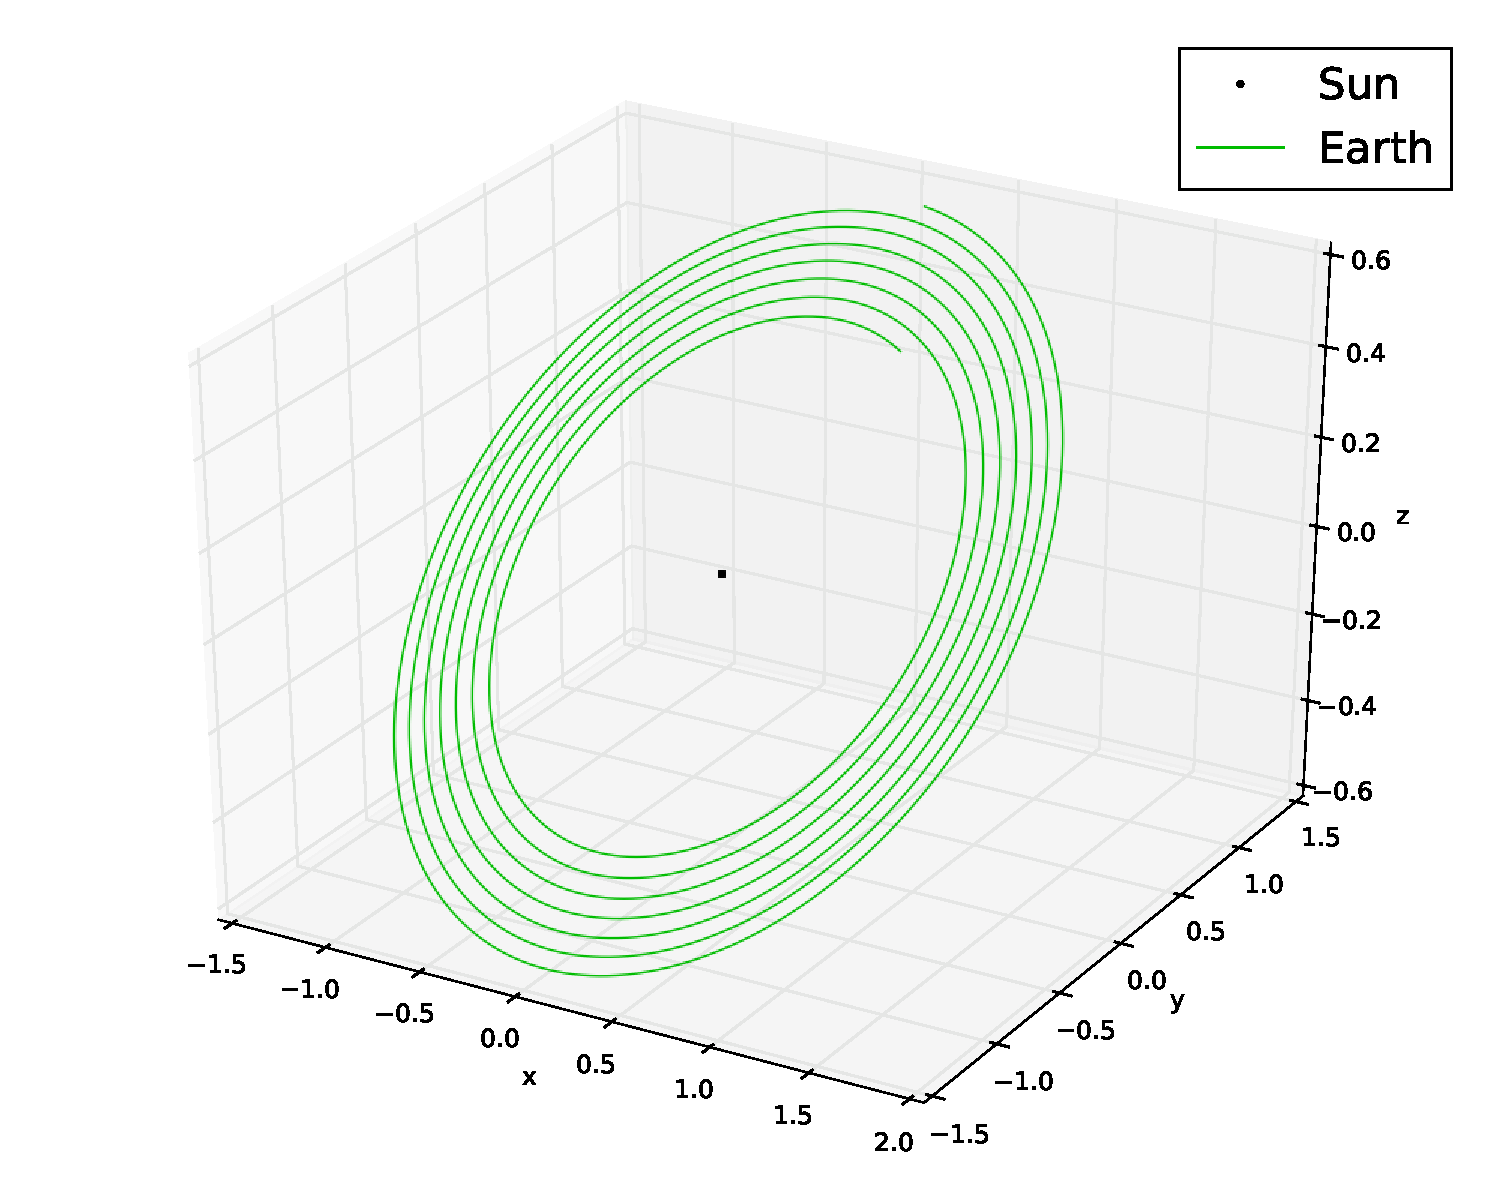
\includegraphics[width=\linewidth]{fig/Two_Bodies_Forward_Euler.pdf}
\caption{Forward Euler}
\label{subfig:2body_euler}
\end{subfigure}
\begin{subfigure}{0.5\textwidth}
\centering
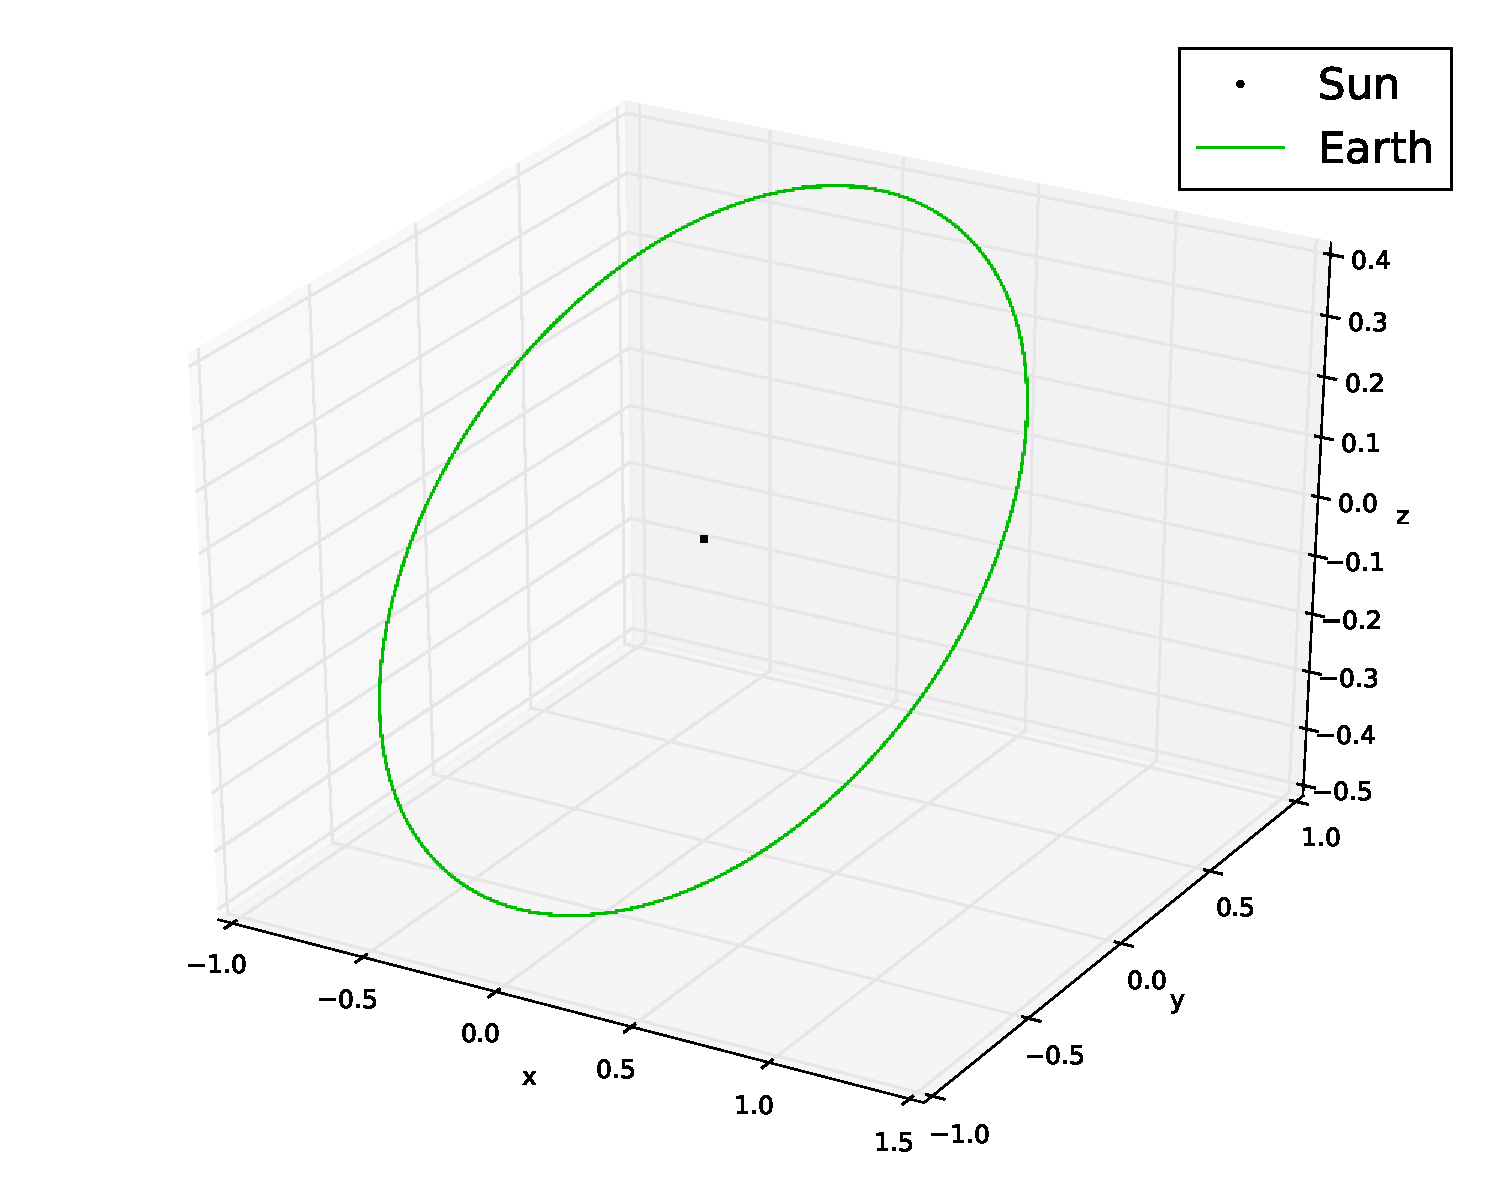
\includegraphics[width=\linewidth]{fig/Two_Bodies_Velocity_Verlet.pdf}
\caption{Velocity Verlet }
\label{subfig:2body_verlet}
\end{subfigure}
\caption{Earth-Sun system solved with the Forward Euler algorithm in (a) and the Velocity Verlet algorithm in (b). The time step is set to 0.001 years and the simulation is run for 10 years for both algorithms.}
\label{fig:2body}
\end{figure}

As shown in \ref{sec:euler} and \ref{sec:verlet}, the local error of the Velocity Verlet algorithm is one order of magnitude smaller than that of the Forward Euler algorithm, and is therefore expected to perform better in terms of precision. In addition, the equations better represents the physical situation by including the acceleration when updating the positions. The Forward Euler algorithm conserved linear momentum fairly well, and is therefore not too bad at updating the velocities. But the algorithm performs poorly when it comes to positions.

The Forward Euler algorithm is slightly faster than the Velocity Verlet algorithm, as expected since updating the positions and velocities requires less floating point operations. There is, however, additional calculations that are needed for both algorithms for each step, such as computing the forces and accelerations. Therefore, computing the new positions and velocities is only a part of the total number of operations needed and the difference between the two algorithms is not as large as might be expected when only comparing the difference in floating point operations of the two algorithms. Table \ref{tab:exec} shows typical execution times for the 2-body problem using the two algorithms for different step sizes. The table indicates that the execution time scale linearly with the number of steps for the two-body problem.  In addition to the computations needed to solve the problem, the positions are written to a file for each step, which also adds a constant overhead in both algorithms in execution times. 

\begin{table}[h]
\centering
\caption{Execution times for the Forward Euler algorithm and the Velocity Verlet algorithm for the two-body problem}
\label{tab:exec}
\begin{tabularx}{\textwidth}{r X r X r }
\hline
n && Forward Euler && Velocity Verlet \\
\hline\hline
$10^2$ && $0.003407$s && $0.004039$s \\
$10^3$ && $0.012861$s && $0.013250$s \\
$10^4$ && $0.078251$s && $0.080261$s \\
$10^5$ && $0.550461$s && $0.613225$s \\
$10^6$ && $4.283050$s && $4.408770$s \\
$10^7$ && $40.80890$s && $42.68170$s \\
$10^8$ && $399.5480$s && $426.0720$s \\
\hline
\end{tabularx}
\end{table}

With a fixed Sun at the origin the theoretical escape velocity, or more correctly escape speed, of the Earth was in equation \ref{eq:esc} shown to be (skipping units) $v=\sqrt{8}\pi\approx8.8857658763$. Figure \ref{fig:esc} shows the simulations of the 2-body problem with the Sun fixed at the origin with different speeds closer and closer to the theoretical escape speed. For smaller speeds the Earth is bound in an elliptical orbit, but as the speed increases the planet goes into a larger and larger elliptical orbit, before it finally turns into a parabola and the Earth escapes. As expected the energy $E=-1.53653\times 10^{-7}$ for $v=8$ is negative, and goes towards zero as the speed goes toward the escape speed. Calculating the Earth's speed for a random sample from \cite{eph} gives a value of $v_{Earth}\approx6.37$, which means the Earth will remain safely in orbit around the Sun.

\begin{figure}
\centering
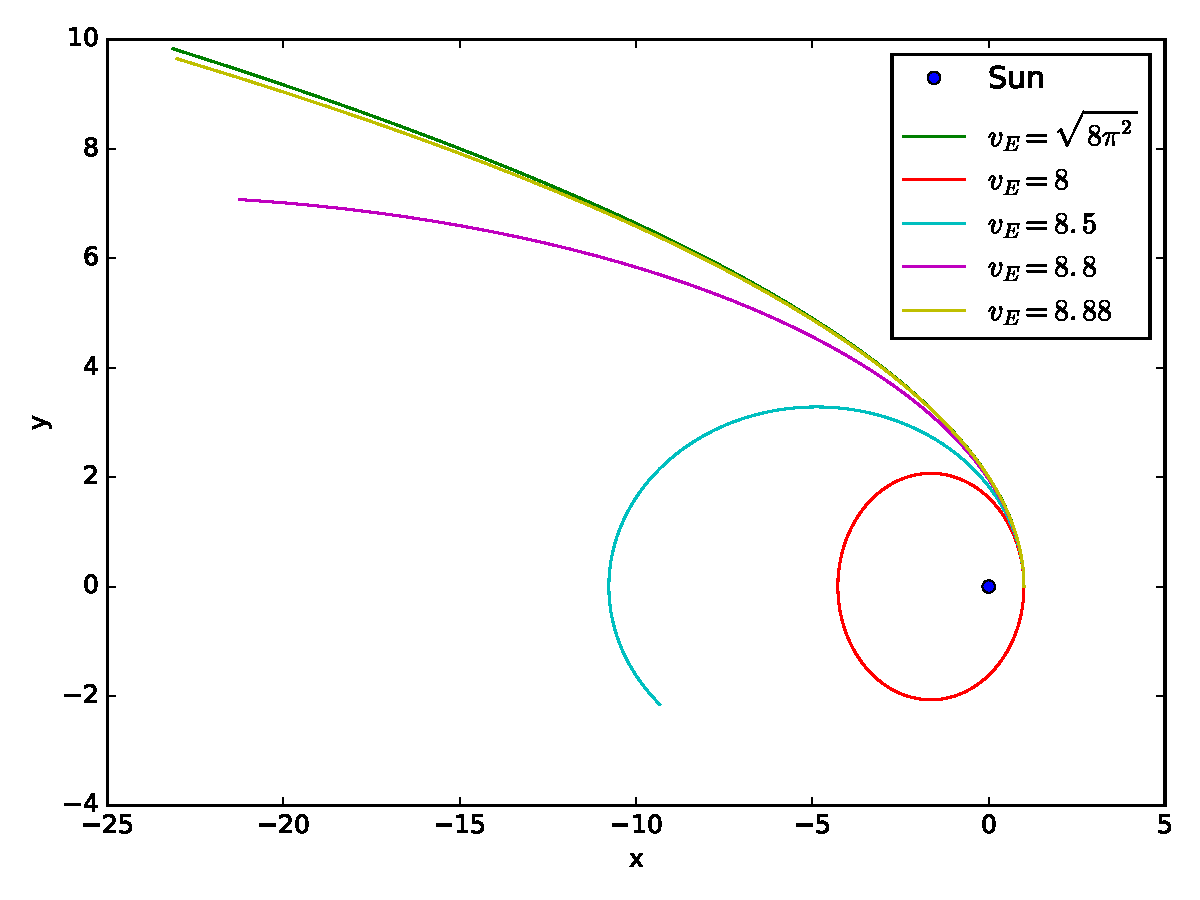
\includegraphics[width=0.8\linewidth]{fig/Two_Bodies_Escape_2D.pdf}
\caption{Earth orbits as Earth's speed approach the theoretical escape speed at $\sqrt{8}\pi$}
\label{fig:esc}
\end{figure}

\FloatBarrier
\subsection{Three-body problem}
Adding Jupiter to the Earth-Sun system, the problem turns into a three-body problem. Jupiter is the largest planet in the solar system and may have an effect on the orbits of other celestial bodies. Using the Velocity Verlet algorithm the Earth-Jupiter-Sun system has been solved both with and without considering the gravitational forces acting on the Sun. The mass of Jupiter has been increased to see how it affects the orbits. Figure \ref{fig:3body} shows the calculated orbits as the mass of Jupiter increases and figure \ref{subfig:3body} shows the three-body problem with normal mass. 
\begin{figure}
\begin{subfigure}[b]{0.5\textwidth}
\centering
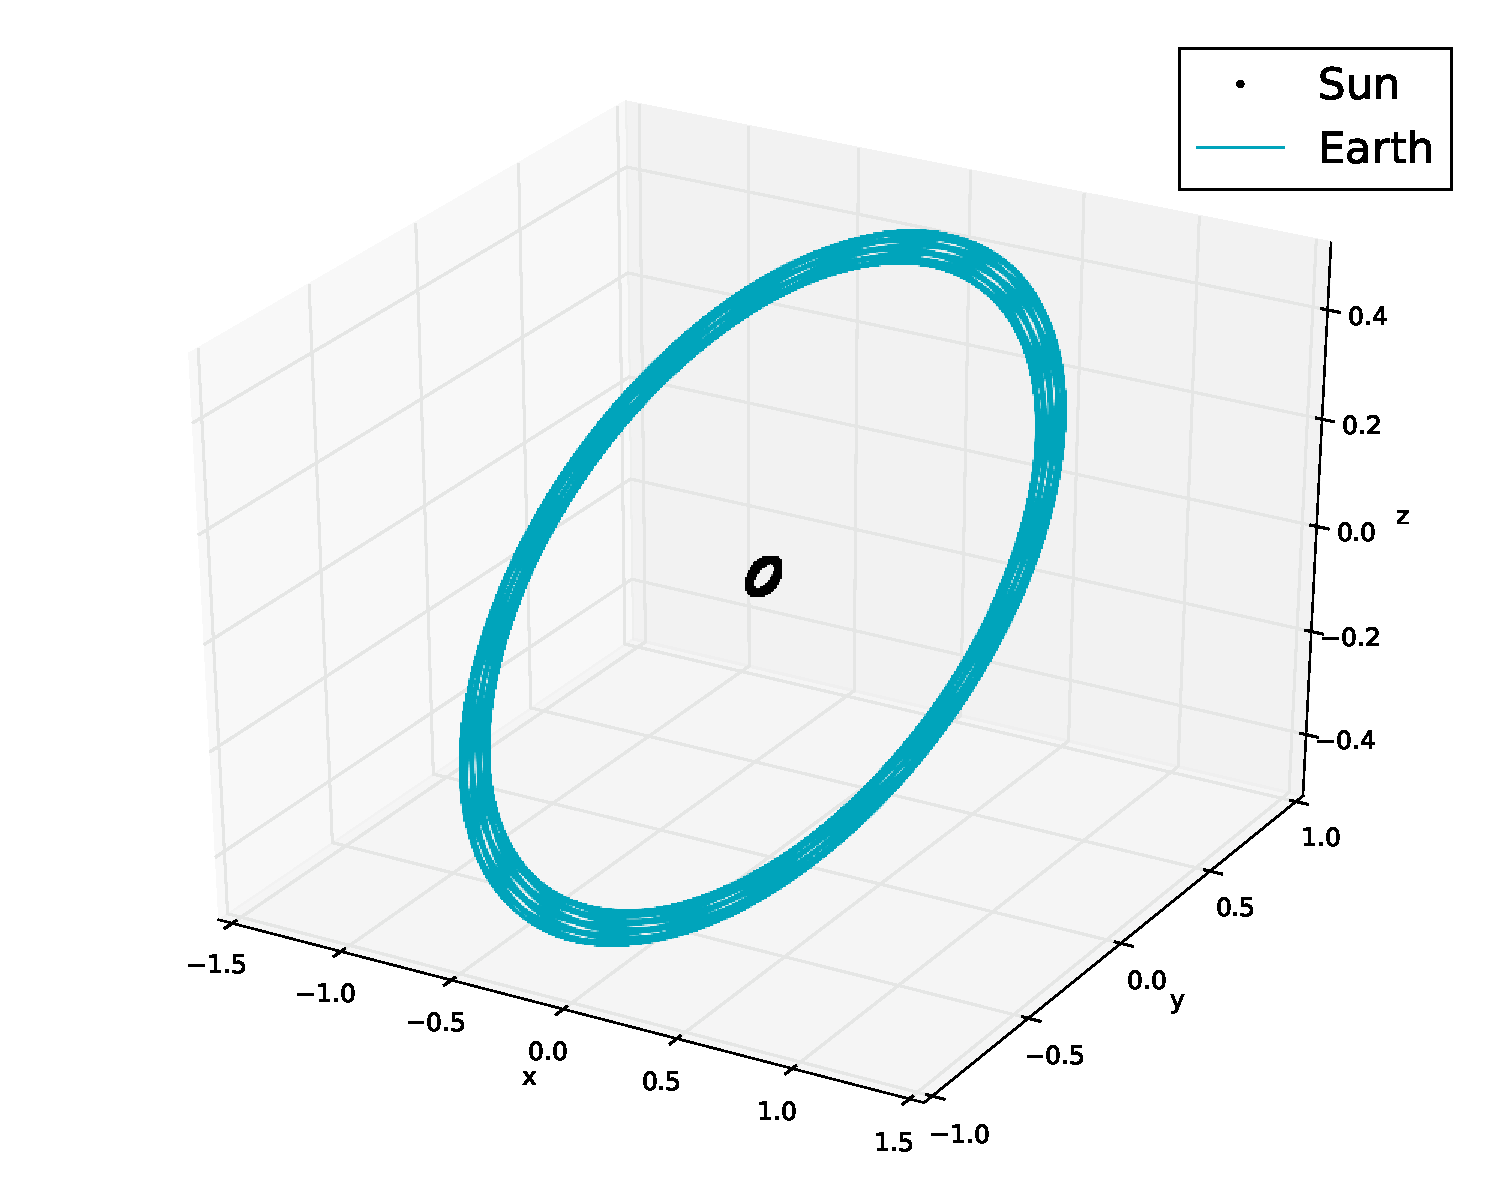
\includegraphics[width=1\linewidth]{fig/Three_Bodies_Big_Jupiter_Earth.pdf}
\caption{Big Jupiter}
\label{subfig:3body_big}
\end{subfigure}
\begin{subfigure}[b]{0.5\textwidth}
\centering
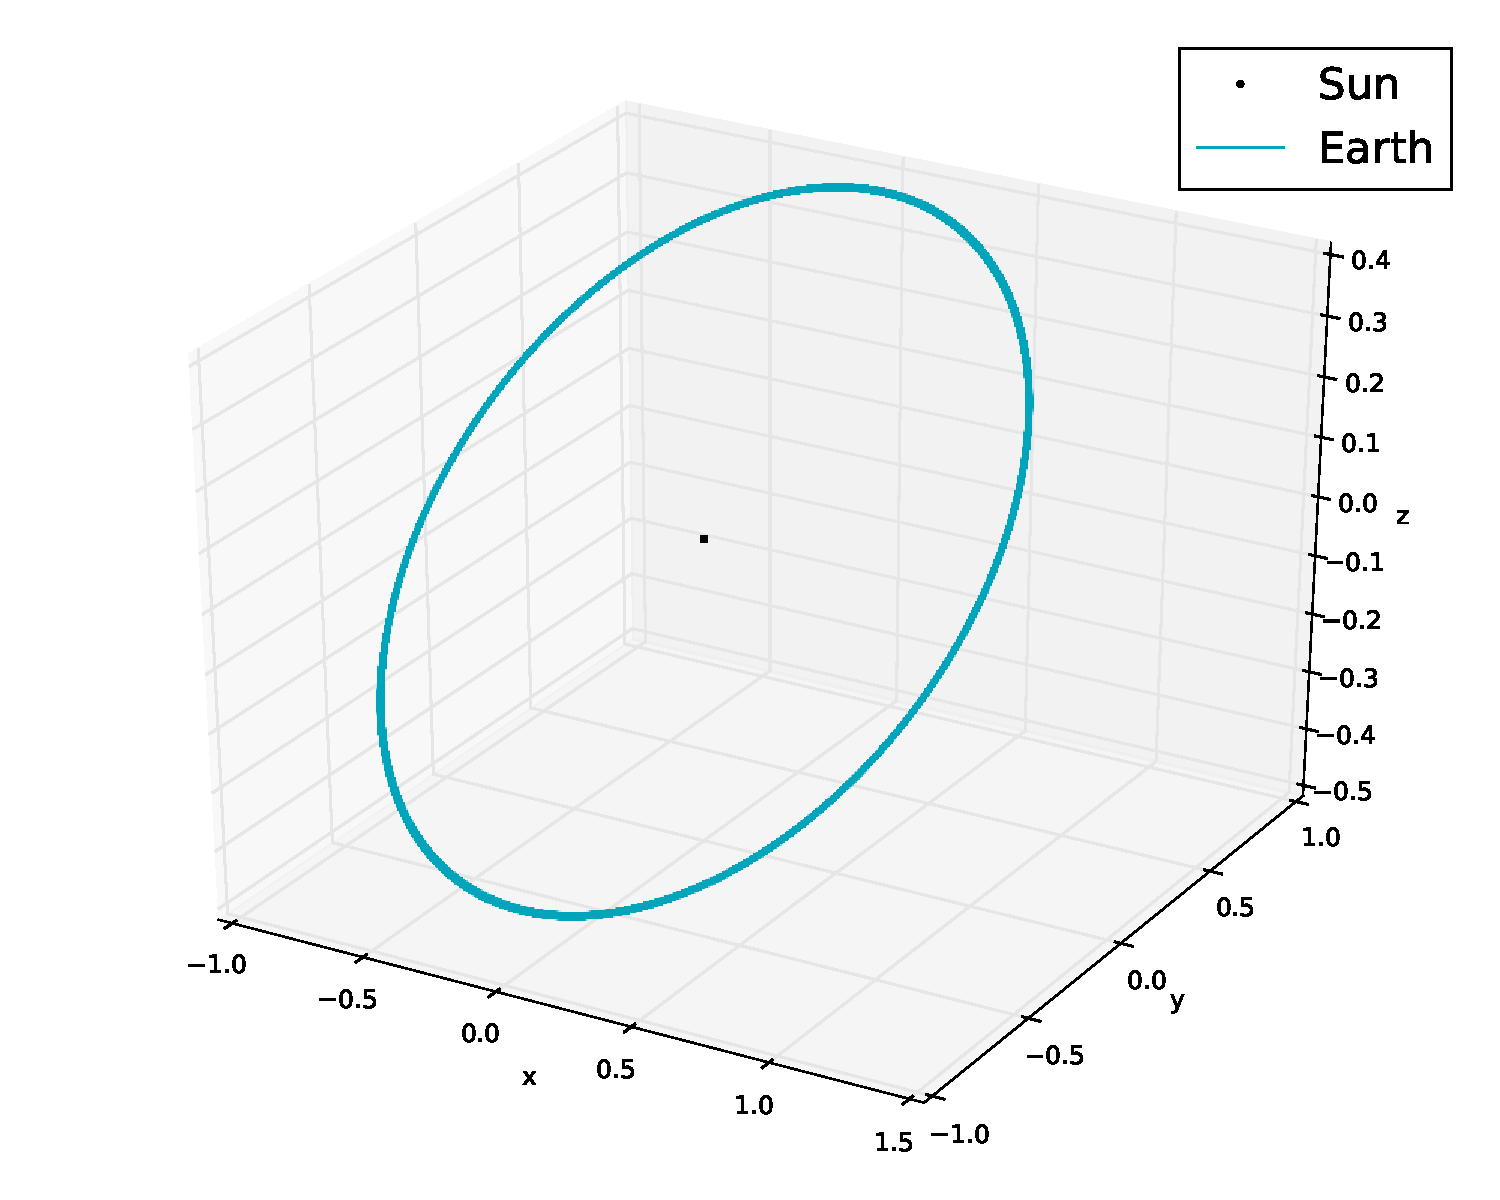
\includegraphics[width=1\linewidth]{fig/Three_Bodies_Big_Jupiter_Fixed_Earth.pdf}
\caption{Big Jupiter, Sun fixed }
\label{subfig:3body_big_fixed}
\end{subfigure}
\begin{subfigure}[b]{0.5\textwidth}
\centering
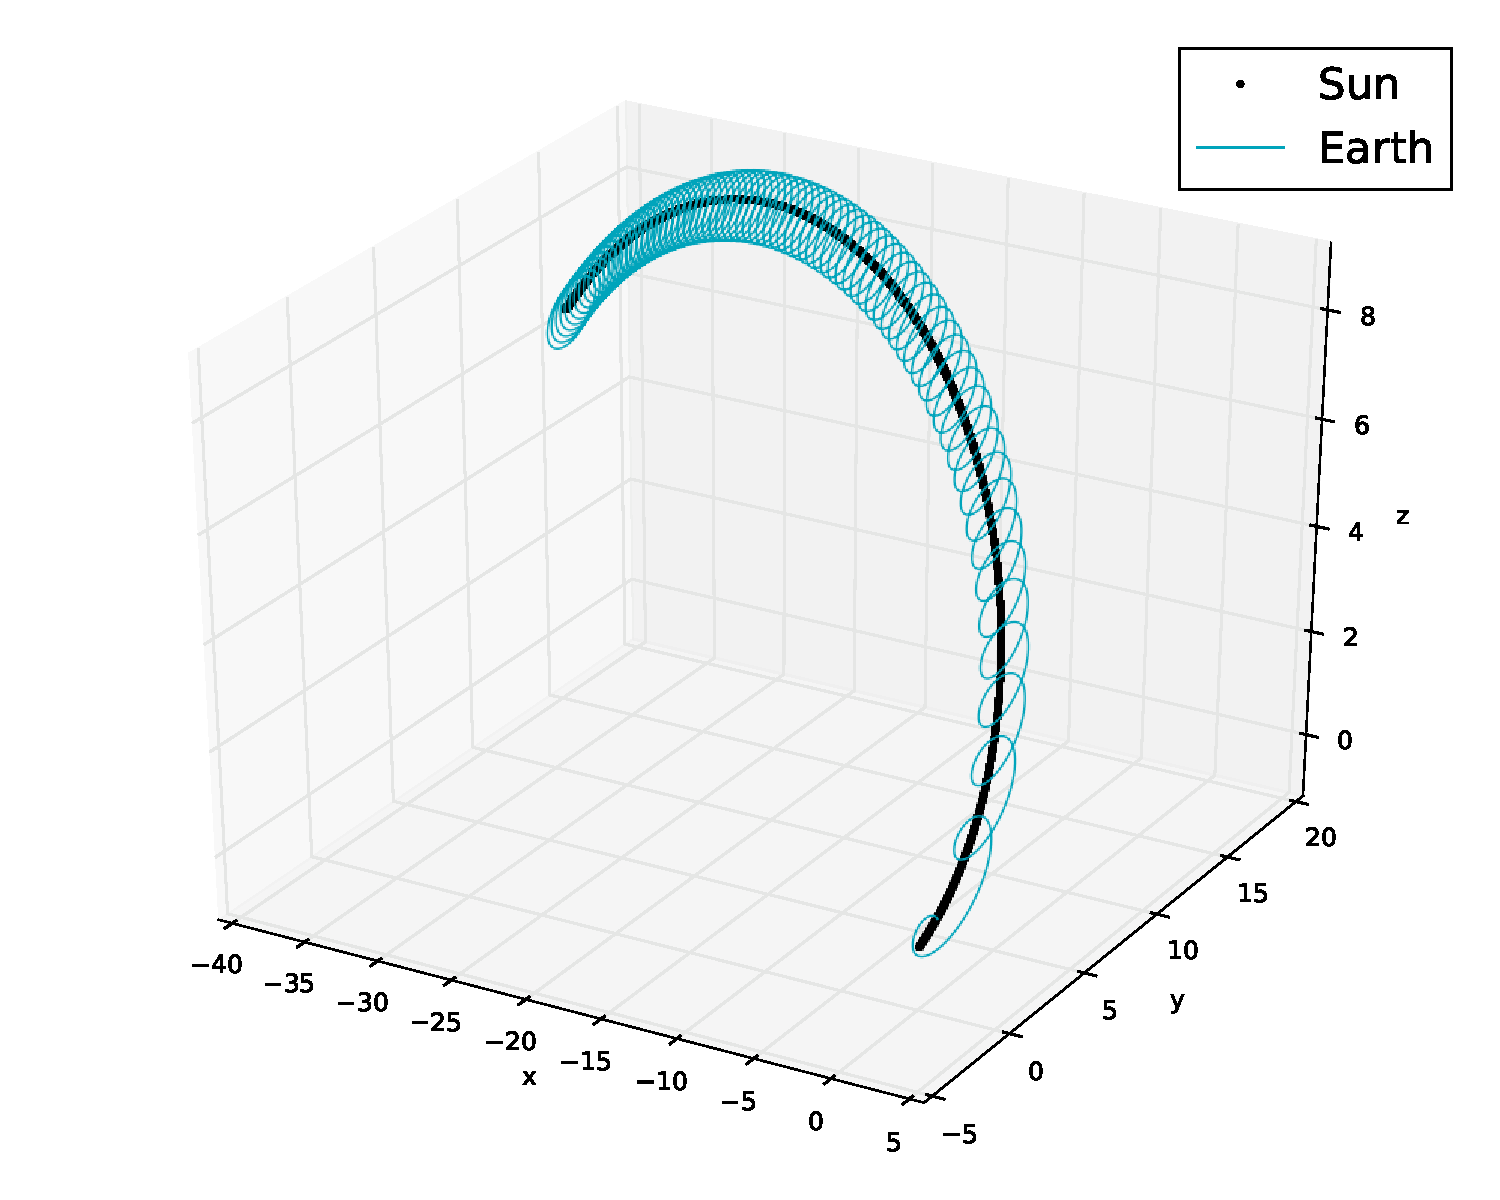
\includegraphics[width=1\linewidth]{fig/Three_Bodies_Huge_Jupiter_Earth.pdf}
\caption{Huge Jupiter}
\label{subfig:3body_huge}
\end{subfigure}
\begin{subfigure}[b]{0.5\textwidth}
\centering
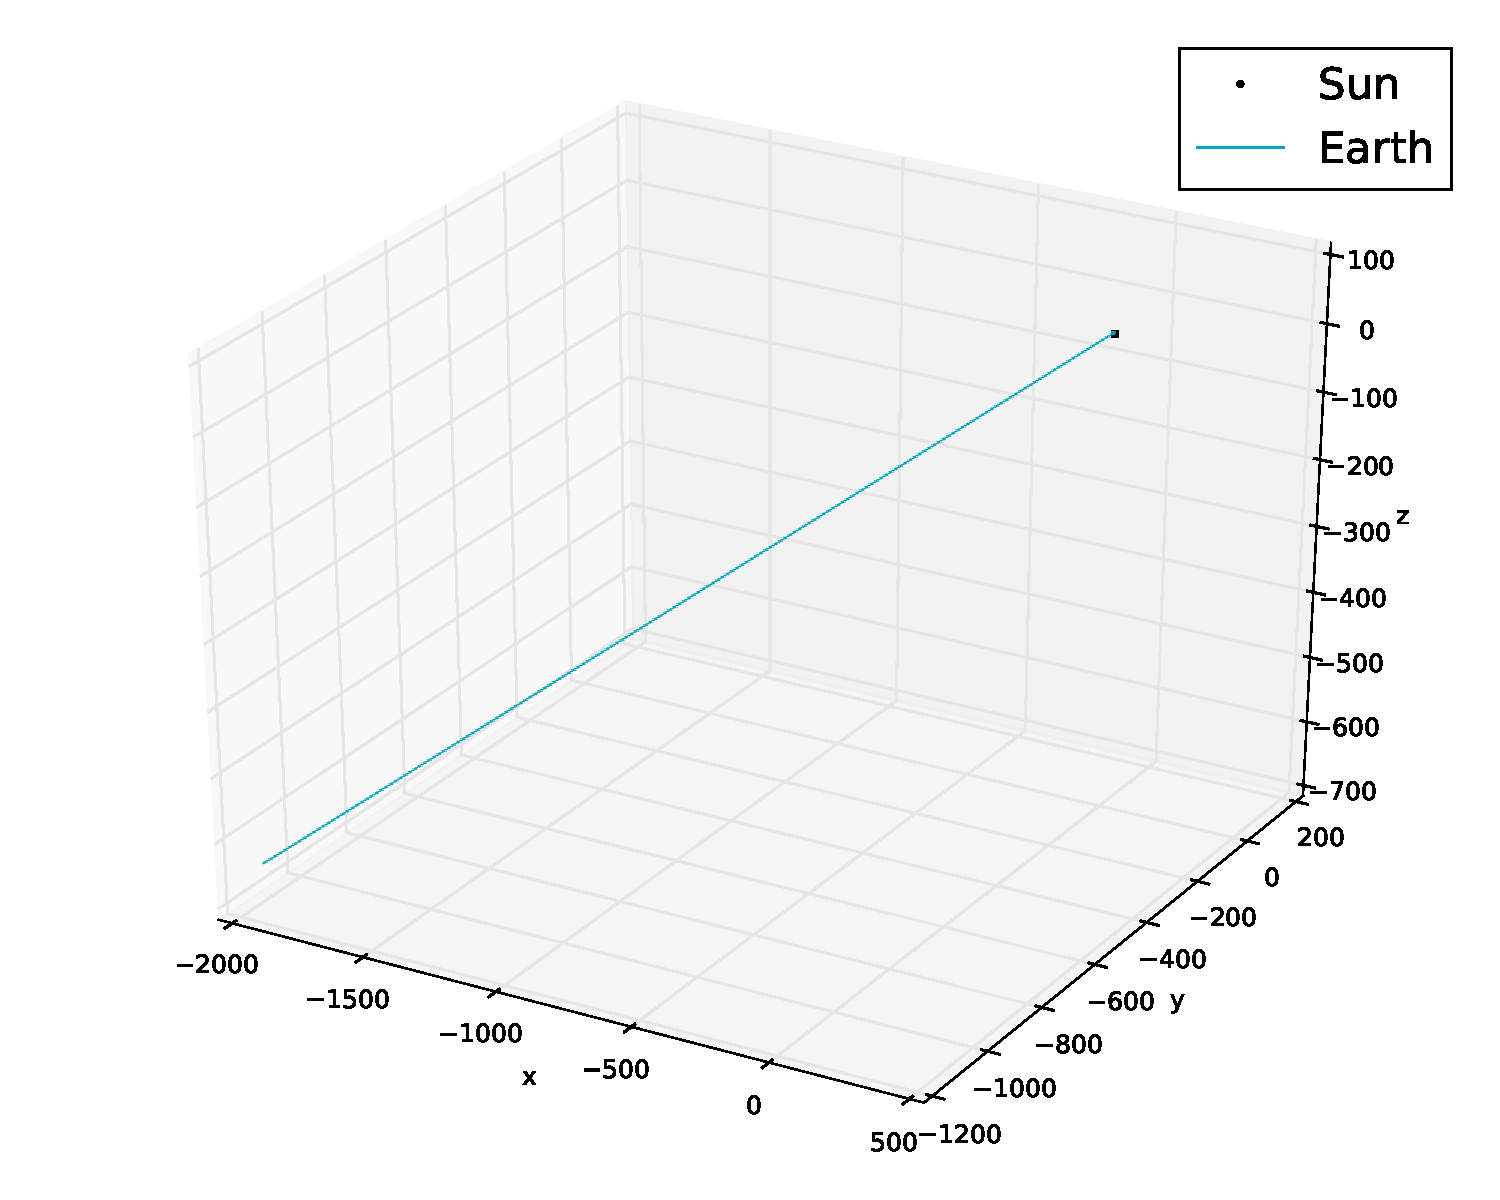
\includegraphics[width=1\linewidth]{fig/Three_Bodies_Huge_Jupiter_Fixed_Earth.pdf}
\caption{Huge Jupiter, Sun fixed}
\label{subfig:3body_huge_fixed}
\end{subfigure}
\caption{Earth-Jupiter-Sun system solved with the Velocity Verlet algorithm. The time step is set to 0.001 years and the simulation is run for 100 years for all cases. The orbit of Jupiter is omitted from the figures. In (a) Jupiter is 10 times its normal mass. In (b) Jupiter is 10 times its normal mass and the sun is fixed at the origin. In (c) Jupiter is 1000 times its normal mass. In (d) Jupiter is 1000 times its normal mass and the sun is fixed at the origin.}
\label{fig:3body}
\end{figure}

As seen in figure \ref{subfig:3body_big_fixed} the Earth's orbit around the Sun is still stable even with the mass of Jupiter being increased by a factor of 10. The perturbations in the orbit due to Jupiter is difficult to see at this scale. However, if the forces on the Sun is also considered, the motion of the Sun due to the gravitational force from Jupiter can be observed. The Sun is approximately 1AU from the Earth while Jupiter is approximately 5.20AU from the Sun and therefore approximately 4.20AU from the Earth when the planets are aligned. The gravitational force falls off as $1/r^2$. Therefore, the main contribution to the change in the orbit of the Earth is not from Jupiter itself, but from the change in the Sun's position due to the gravitational force from Jupiter, as can be seen in figure \ref{subfig:3body_big}. 

Increasing the mass of Jupiter further, with a factor of 1000, the system becomes unstable for the fixed Sun and the Earth escapes the solar system. Assuming the Sun is not affected by the gravitational force from the planets is clearly a poor approximation now that Jupiter's mass is of the same order of magnitude as the Sun's mass. This is shown in figure \ref{subfig:3body_huge_fixed}. A smaller step size is needed to capture the complicated motions of the Earth when the Sun is fixed. If the gravitational forces acting on the Sun is considered the solution again becomes stable, as seen in figure \ref{subfig:3body_huge}. The Sun and Jupiter start orbiting the system's new center of mass and the Earth follows in orbit around the Sun.

\begin{figure}
\begin{subfigure}[b]{0.5\textwidth}
\centering
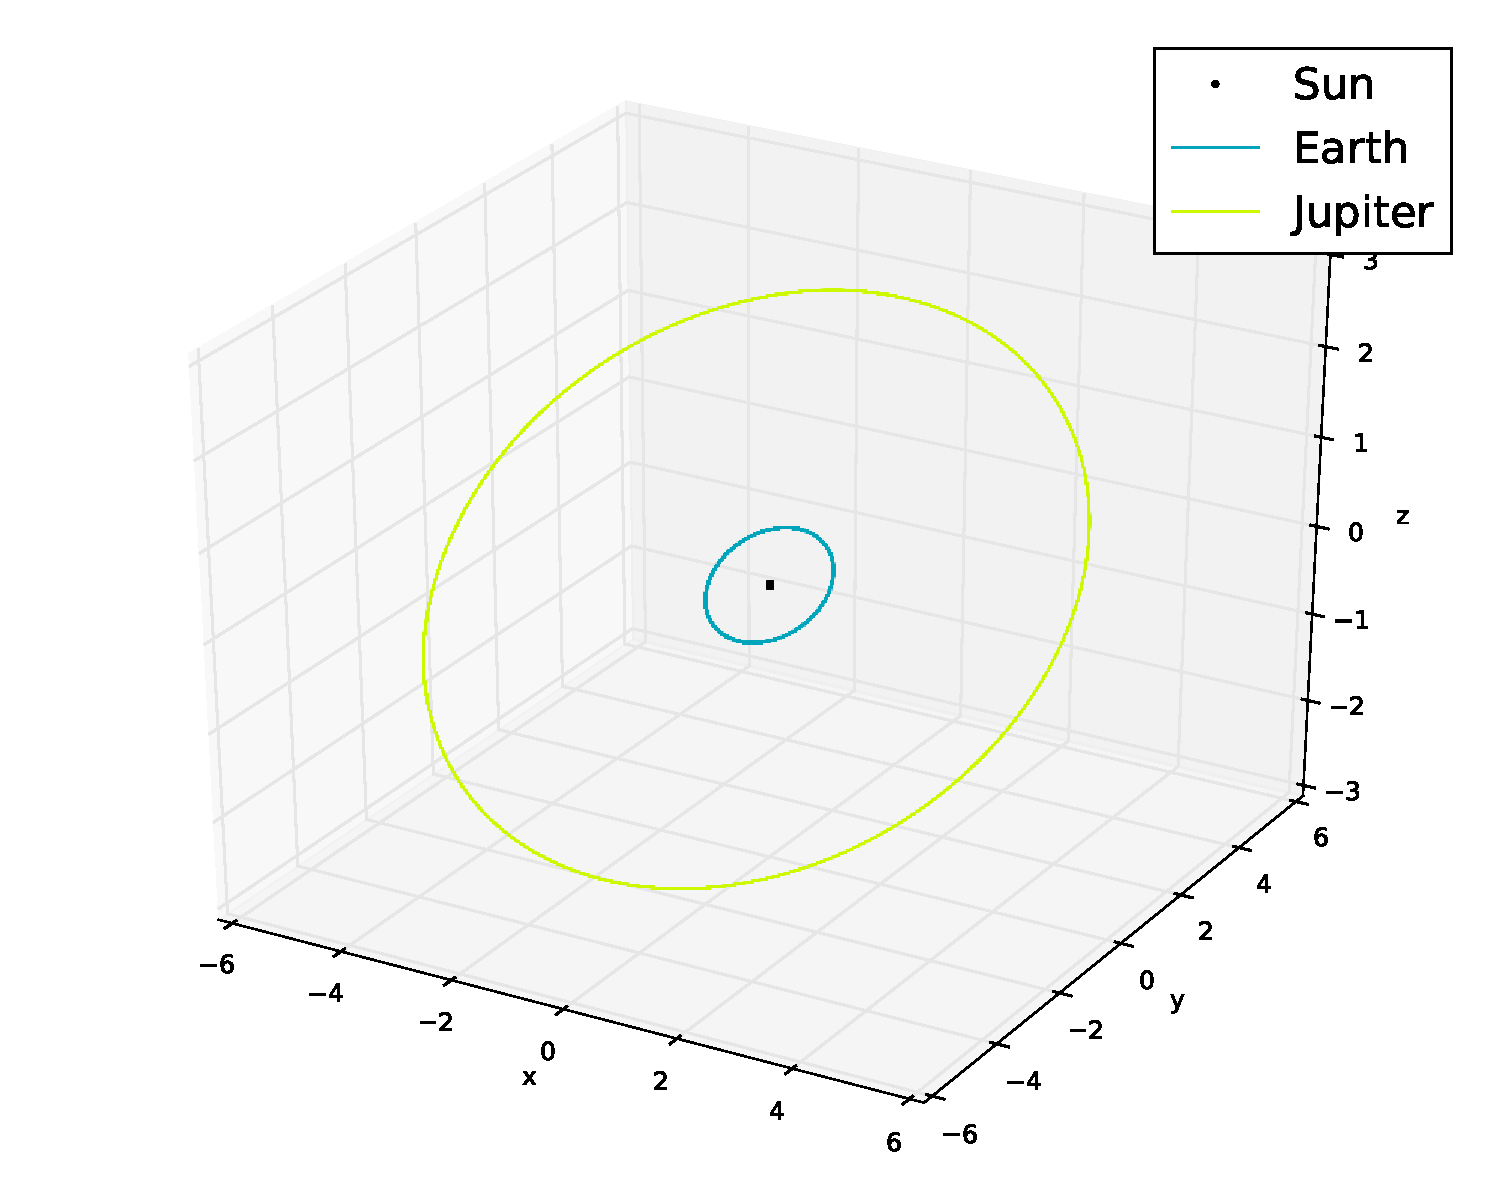
\includegraphics[width=1\linewidth]{fig/Three_Bodies.pdf}
\caption{Three-body problem}
\label{subfig:3body}
\end{subfigure}
\begin{subfigure}[b]{0.5\textwidth}
\centering
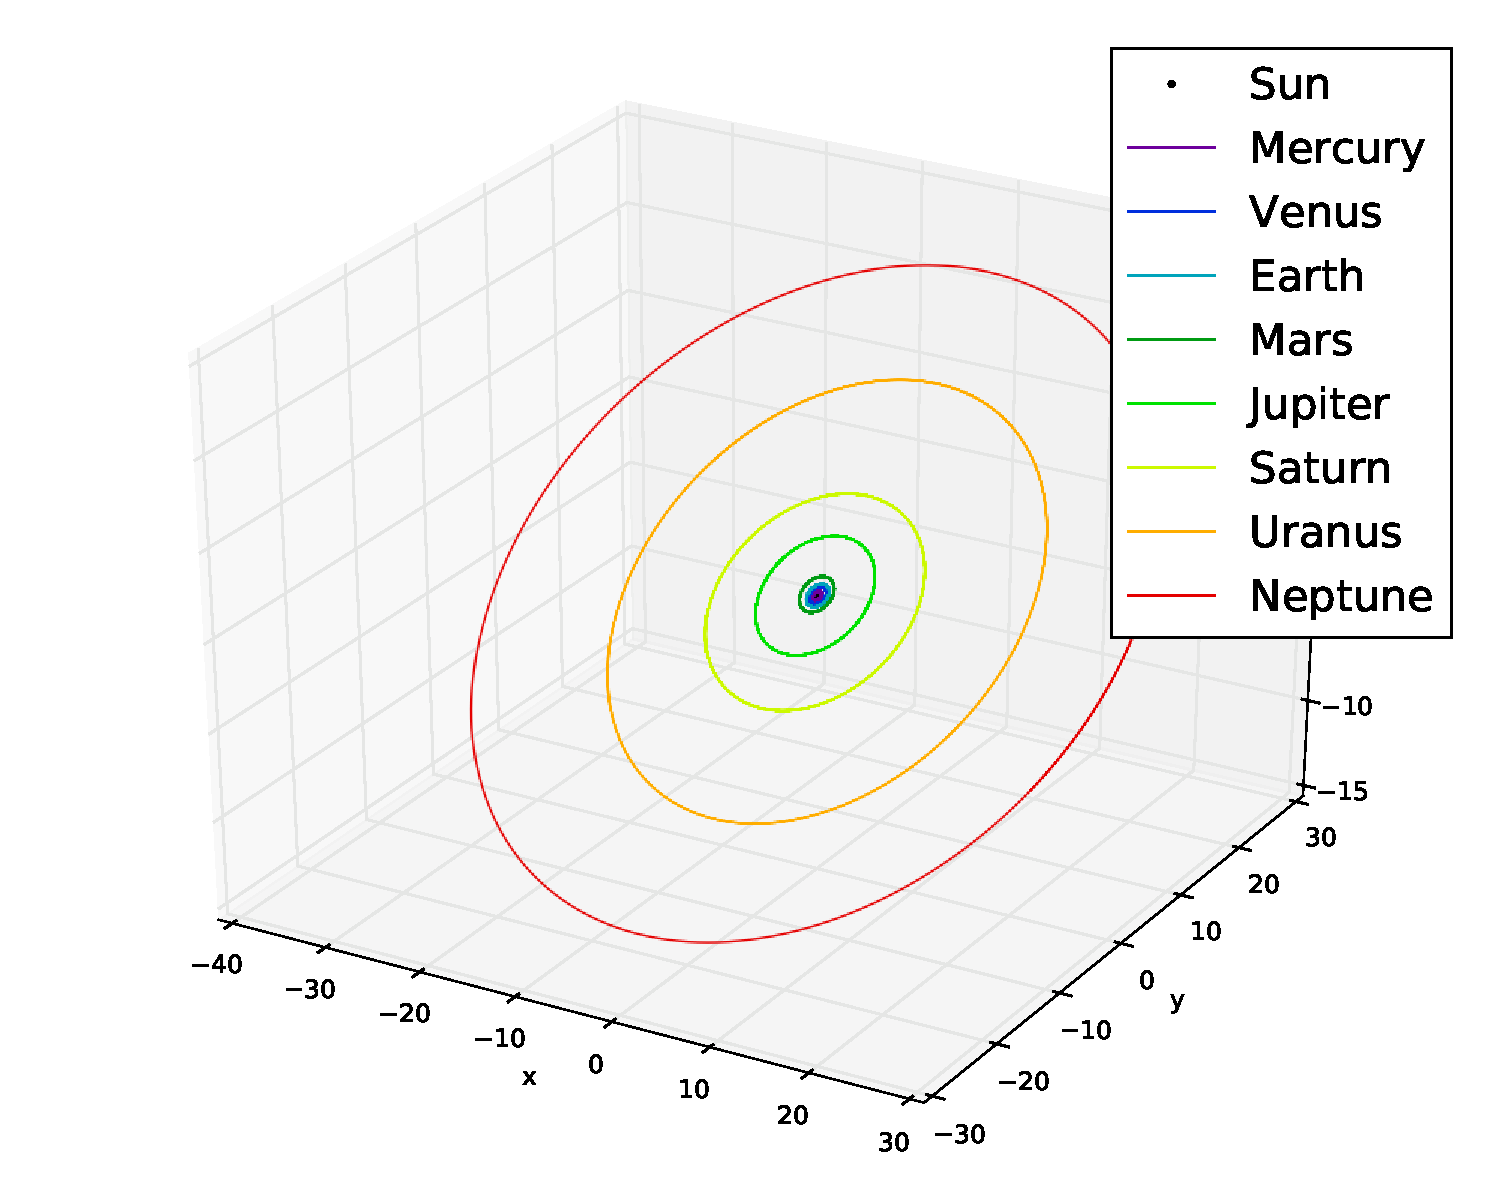
\includegraphics[width=1\linewidth]{fig/Solar_System.pdf}
\caption{9-body problem}
\label{subfig:9body}
\end{subfigure}
\begin{subfigure}[b]{0.5\textwidth}
\centering
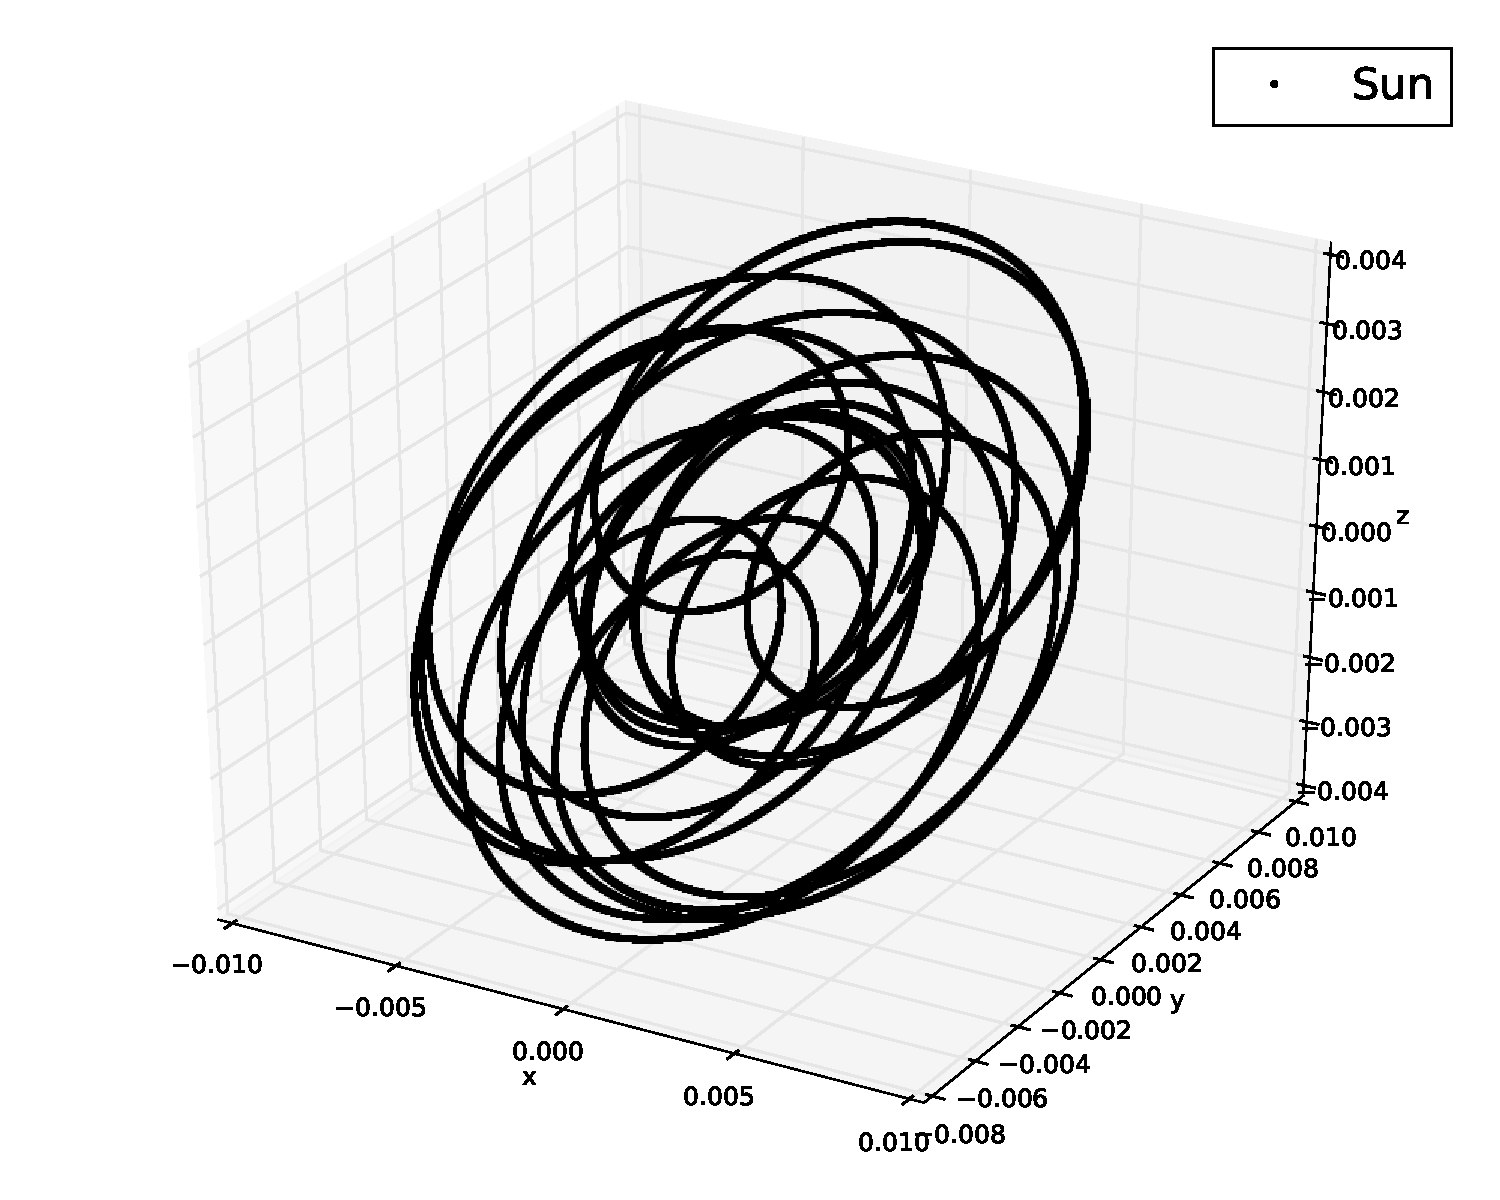
\includegraphics[width=1\linewidth]{fig/Solar_System_Sun.pdf}
\caption{9-body problem}
\label{subfig:9body_sun}
\end{subfigure}
\begin{subfigure}[b]{0.5\textwidth}
\centering
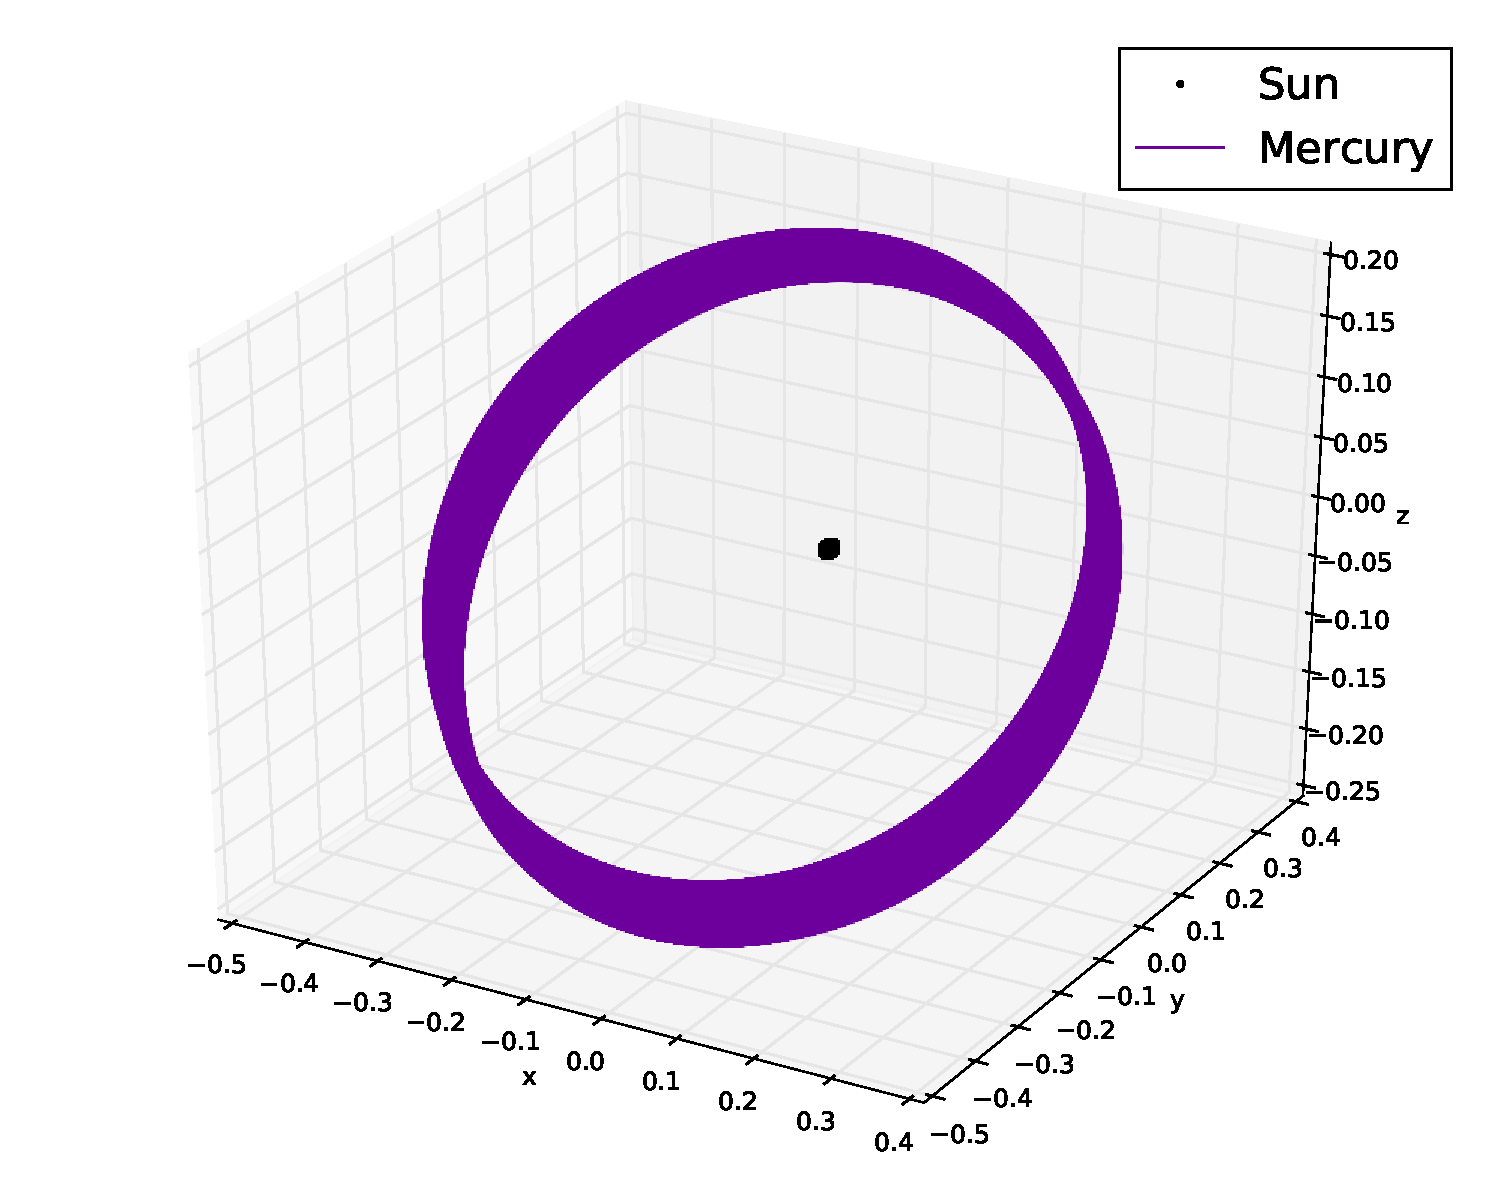
\includegraphics[width=1\linewidth]{fig/Solar_System_Mercury.pdf}
\caption{9-body problem}
\label{subfig:9body_mercury}
\end{subfigure}
\caption{N-body system solved with the Velocity Verlet algorithm with initial position and velocities from \cite{eph}. Gravitational forces on the Sun is included. In (a) the time step is set to 0.001 years and the simulation is run for 10 years. In (b) the time step is set to 0.001 years and the simulation is run for 200 years. (c) shows the orbit of the Sun from the solution in (b) and (d) shows the orbit of Mercury from the solution in (b).}
\label{fig:Nbody}
\end{figure}

Finally, adding all the planets in the solar system the problem becomes a 9-body problem. The planet furthest away from the Sun is Neptune with a orbital period of approximately 164 years. To get a full revolution of all the orbits a solar system simulation is run with a duration of 200 years and with time step 0.001. The results are shown in \ref{subfig:9body}. Even with this crude time step and 9 bodies the Velocity Verlet algorithm produces stable orbits for all the celestial bodies. In figure \ref{subfig:9body_sun} the influence of the other planets on the Sun can be seen but compared to the radius of the Sun at approximately 0.0047AU the motion is not very large. In figure \ref{subfig:9body_mercury} the precession of Mercury's orbit due to the gravitational force of the other planets can be seen.

\FloatBarrier
\subsection{Mercury's perihelion precession}

Removing the effect on Mercury's orbit from the gravitational force from the other planets there is still some part of the observed precession that is unaccounted for. By using the modified Newtonian gravitational force in \ref{eq:grav_gr} and solving the two-body problem of the Mercury-Sun system this effect can be seen. Starting with Mercury at perihelion at $t_0$ and with $\bm{x}_0=(0.3075AU, 0, 0)$ and $\bm{v}_0=(0, 12.44AU/year, 0)$, the perihelion angle can be calculated as $\theta_p = \arctan{(y_p/x_p)}$, where $x_p$ and $y_p$ is the $x$ and $y$ coordinate of the perihelion. This motion is 2-dimensional and the z-coordinate is ignored. With $r^2 = x_p^2 + y_p^2$, finding the perihelion positions is the problem of finding all the minimum values of $r$ over the duration of the simulation. This is done and figure \ref{fig:peri} shows how the perihelion angle changes over time. The simulation is run with a time step of $h=10^{-6}$ and a duration of 100 years. The time step is not small enough to determine the perihelion position with high precision, which causes the fluctuations seen in the figure, but it is small enough to see the trend. The theory of general relativity predicts a perihelion precession of 43$''$ per century, as described in section \ref{sec:gr}, which is approximately 0.01194 degrees. The simulation clearly shows a linear trend in the perihelion precession and the value over one century is close to 43$''$. 

\begin{figure}
\centering
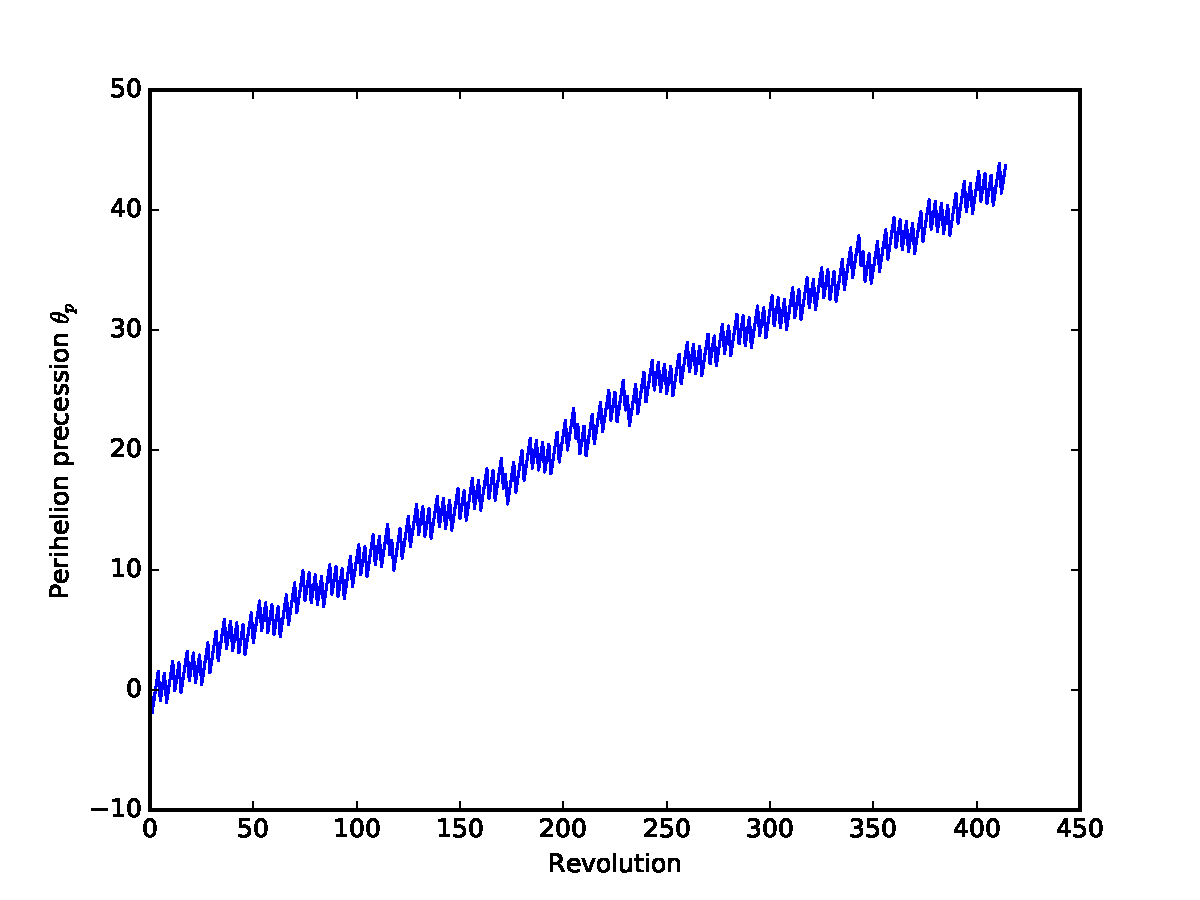
\includegraphics[width=0.8\linewidth]{fig/Perihelion_Precession.pdf}
\caption{Angular change in arc seconds in Mercury's perihelion for each revolution around the Sun for a simulation run over 100 years.}
\label{fig:peri}
\end{figure}

\section{Conclusions}
\label{sec:conclusions}
For simulating the orbital motion of celestial bodies in the solar system the Velocity Verlet algorithm is superior to the Forward Euler algorithm. The Forward Euler algorithm is slightly faster and easier to implement, but the Velocity Verlet algorithm produces more stable orbits for step size $h=10^{-2}$ than the Forward Euler algorithm does for step size $h=10^{-7}$.

The Sun is the by far most important contributor to the planets' orbits, but the planets also have an effect on the motion of the Sun. The Sun orbits the solar system's center of mass, and the orbital motion is of the same order of magnitude as the Sun's radius. The planets also have a smaller effect on each other, with the most visible effect on Mercury. Mercury's precessing orbit seems to be a combination of the gravitational effect from the other planets and the theory of general relativity.


\clearpage

\begin{thebibliography}{1}
\bibitem{lectures} Hjort-Jensen, M., 2015. Computational physics. Available at https://github.com/CompPhysics/ComputationalPhysics/
\bibitem{physics} Young, Freedman, Sears and Zemansky's University Physics with Modern Physics, 11th edition, Addison-Wesley, 2004  
\bibitem{framework} https://github.com/mortele/solar-system-fys3150. Framework for implementation
\bibitem{horizon} http://ssd.jpl.nasa.gov/horizons.cgi Jet Propulsion Laboratory - Horizons web interface
\bibitem{eph} ftp://ssd.jpl.nasa.gov/pub/eph/planets/bsp Jet Propulsion Laboratory - Ephemerides files
\bibitem{jplephem} https://pypi.python.org/pypi/jplephem - Parser for ephemerides files
\end{thebibliography}





\end{document}
